\noindent
\large {\bf Genotyping somatic insertions and deletions} 


\normalsize 


\noindent \paragraph{Keywords:} Cancer Genomes, Insertions and Deletions, Next-Generation Sequencing Data, Precision
Oncology, Somatic Variants, Data Uncertainty

\noindent \paragraph{Abstract:} 


Cancer is a genetic disorder in the first place; somatic mutations in the genome of an originally healthy cell allow for the maintenance of a potentially rapidly proliferating hetergeneous mix of cancer
clones. This explains why in the recent past several thousands of cancer/control genome pairs have been
sequenced, concerted by global consortia [7]; to date, the cancer genomes sequenced already amount to
petabytes of data. The promises this massive pile of data holds for applications in precision oncology are
enormous and have the potential to lead to drastically improved diagnosis and selection of therapy protocols.

While calling somatic single nucleotide variants (SNVs) can be done at both high recall and precision
(e.g. [1, Mutect]), calling somatic indels has remained difficult and complex. Confounding factors, such as
alignment and fragment length uncertainty, can pose substantial challenges already for germline indels. This
becomes particularly disturbing for indels of length 30-150 bp (the NGS twilight zone of indels). In earlier
work, we have shown how to resolve these issues and safely call and genotype substantial amounts of such
indels in the frame of population-scale projects [4, 3, 5].

When calling and genotyping somatic indels, where genotyping refers to estimating the allele frequency
of variants, cancer heterogeneity and data impurity make another confounding layer of issues. Heterogeneity and impurity of samples imply that estimating the allele frequency of somatic variants requires to
appropriately quantify the inherent uncertainties. Only if this complex mix of disturbing factors has been
appropriately disentangled, calling somatic indels at sufficient recall and precision is possible. Since, prior
to our approach, there have been no methods to call somatic twilight zone indels, somatic variant databases
are still virtually devoid of this type of genetic variation. Beyond this, genotyping somatic indels has also
remained a substantial computational challenge in general.

Here, we present a method, PROSIC (Postprocessing somatic indel calls), based on a Bayesian
latent variable model (see Fig. 1) that aids in genotyping somatic indel calls while accounting for the above
mentioned confounding factors of impurity, the unknown clonal structure, and alignment and typing uncertainty. Our method requires a list of potential somatic indel calls in VCF format, together with a cancer
1and a matched normal BAM file as input. The output then is an annotated VCF where indel calls have been
genotyped (by a VAF estimate) and been equipped with a Bayesian type a posteriori probability that the
indel is somatic, as derived from the model.

\begin{figure}[htb]
\begin{center}
        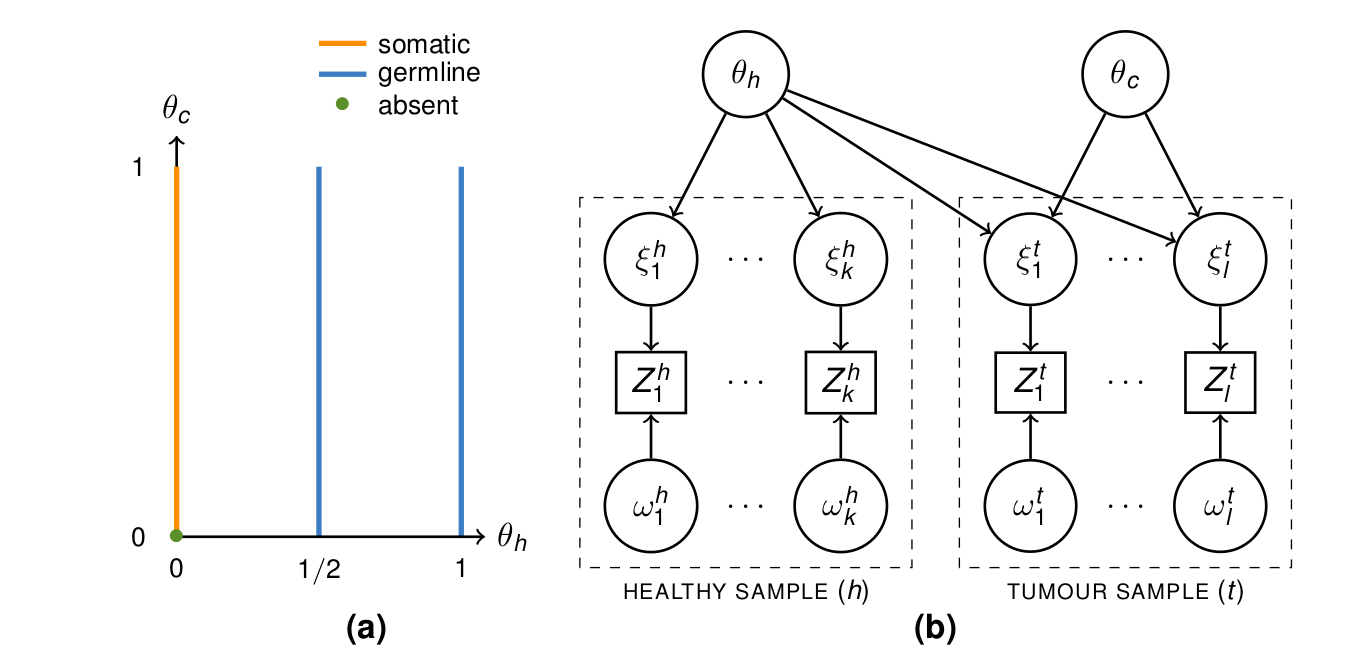
\includegraphics[scale=0.3]{all/13.png}
\label{fig:fig}
\caption{(a) Genotype space. Genotypes need to be estimated for both cancer ($\theta_c$) and control sample ($\theta_h$). While
$\theta_h\in \{0, \frac{1}{2} , 1\}$, representing absence, hetero- or homozygosity of the variant, $\theta_c\in [0, 1]$, reflecting that
VAF’s of somatic variants can cover the whole range due to cancer heterogeneity and impurity. (b) The
latent variable model, where $i\in\{1, \ldots, k\}, ~j\in\{1, \ldots, l\}$ index the alignments of the healthy and the cancer
sample, respectively. Latent variables representing uncertainties ($\omega$, $\xi$) and allele frequencies ($\theta_h,\theta_c$) are
represented by circles; note that $\theta_h$ has an influence also on the cancer sample, which addresses impurity.
Rectangles represent variables ($Z^i_j$) that can be immediately observed, such as alignment length and gaps.}
\end{center}
\end{figure}

We have evaluated our model on simulated data and on the datasets provided by the DREAM challenge
(see \url{https://www.synapse.org/#!Synapse:syn312572}). We demonstrate that we can raise
both recall and precision substantially, often achieving quite drastic improvements (more than 30\% in recall and 30-40\% in precision, reaching precision rates of 85-95\%) in comparison to standard, best-practice
somatic indel calling workflows provided by gold standard indel discovery methods such as Platypus [6],
Pindel [8] and the HaplotypeCaller [2]. We also demonstrate that our tool compares very favorably with
best practice pipelines on cancer/control cell line data. Finally, we point out ways how to substantially
increase recall in the somatic indel twilight zone of 30-150 bp at precison rates of at least 80\% which, to
the best of our knowledge, is novel. The German Cancer Research Center (DKFZ) has submitted an official proposal that our tool will be integrated into the ICGC somatic indel calling pipelines to postprocess
and genotype indel calls arising from the latest TCGA project (\url{https://tcga-data.nci.nih.gov/tcga/tcgaAbout.jsp}) on more than 2800 matched cancer/control genome pairs.

We present a statistical, latent variable model which allows to estimate allele frequencies
of indels in matched cancer/control samples, and to derive Bayesian a posteriori probabilities for the indel
calls to be somatic. In this, we take all disturbing data uncertainties, such as sample impurity, cancer
heterogeneity, alignment and typing uncertainties into account, which also allows us to make good calls
in relatively difficult-to-access regions of the human genome. When applying our model to indel callsets
generated by gold standard indel discovery tools, we achieve substantial improvements over current best-
practice workflows both in terms of recall and precision. In summary, we are providing a tool that allows
to leverage ordinary, well-approved indel callers into high quality somatic indel callers. See \url{https://github.com/louisdijkstra/somatic-indel-calling} for software.


\noindent
\paragraph{References} 
\noindent \paragraph{} 

\noindent 
[1] K. Cibulskis, M.S. Lawrence, S.L. Carter, A. Sivachenko, D. Jaffe, C. Sougnez, S. Gabriel, M. Meyerson, E.S. Lander, and G. Getz. Sensitive detection of somatic point mutations in impure and heterogeneous cancer samples. Nature Biotechnology, 2013.\\

\noindent
[2] Mark A DePristo, Eric Banks, Ryan Poplin, Kiran V Garimella, Jared R Maguire, Christopher Hartl,
Anthony A Philippakis, Guillermo del Angel, Manuel A Rivas, Matt Hanna, Aaron McKenna, Tim J
Fennell, Andrew M Kernytsky, Andrey Y Sivachenko, Kristian Cibulskis, Stacey B Gabriel, David
Altshuler, and Mark J Daly. A framework for variation discovery and genotyping using next-generation
DNA sequencing data. Nature Genetics, 43(5):491–498, May 2011.\\

\noindent
[3] The Genome of the Netherlands Consortium. Whole-genome sequence variation, population structure
and demographic history of the Dutch population. Nature Genetics, 2014.\\

\noindent
[4] Hehir-Kwa et al. A high-quality reference panel reveals the complexity and distribution of structural
genome changes in a human population. Technical report, bioRxiv:036897, 2016.\\

\noindent
[5] Tobias Marschall, Iman Hajirasouliha, and Alexander Schonhuth. MATE-CLEVER: Mendelian-inheritance-aware discovery and genotyping of midsize and long indels. Bioinformatics, 29(24):3143-3150, 2013.\\

\noindent
[6] A. Rimmer, H. Phan, I. Mathieson, Z. Iqbal, S.R.F. Twigg, WGS500 Consortium, A.O.M. Wilkie,
G. McVean, and G. Lunter. Integrating mapping-, assembly- and haplotype-based approaches for calling
variants in clinical sequencing applications. Nature Genetics, 2014.\\

\noindent
[7] The International Cancer Genome Consortium. International network of cancer genome projects. Nature, 464(7291):993–998, 2010.\\

\noindent
[8] Kai Ye, Marcel H. Schulz, Quan Long, Rolf Apweiler, and Zemin Ning. Pindel: a pattern growth
approach to detect break points of large deletions and medium sized insertions from paired-end short
reads. Bioinformatics, 25(21):2865–2871, Nov 2009.


\noindent \paragraph{Authors:} 

